\documentclass[border=6pt]{standalone}
\usepackage{amsmath}
\usepackage{amssymb}
\usepackage{tikz}
\usepackage{xcolor}
\usetikzlibrary{arrows.meta,calc,positioning,shapes.geometric}
\begin{document}
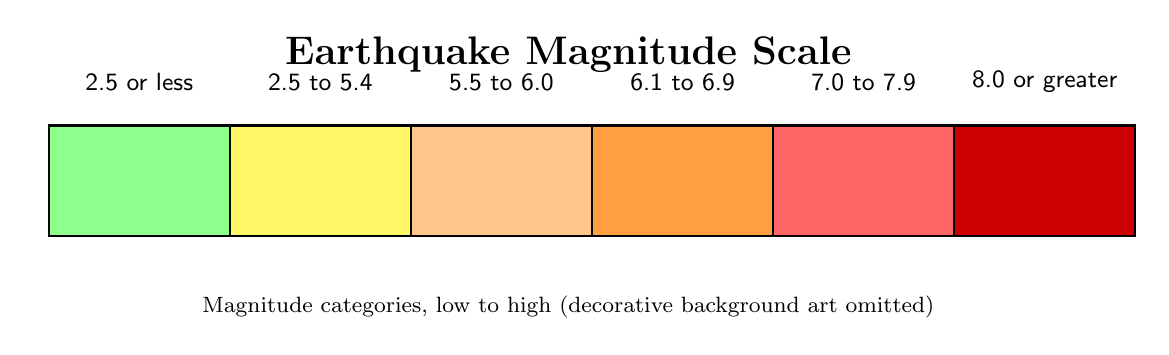
\begin{tikzpicture}[font=\sffamily\small]
  \node[font=\Large\bfseries] at (6.6,2.3) {Earthquake Magnitude Scale};

  \foreach \i/\lbl/\clr in {%
    0/{2.5 or less}/green!45,%
    1/{2.5 to 5.4}/yellow!60,%
    2/{5.5 to 6.0}/orange!45,%
    3/{6.1 to 6.9}/orange!75,%
    4/{7.0 to 7.9}/red!60,%
    5/{8.0 or greater}/red!80!black%
  }{
    \pgfmathsetmacro{\x}{\i*2.3}
    \draw[fill=\clr, thick] (\x,0) rectangle ++(2.3,1.4);
    \node[align=center, text width=2.2cm] at (\x+1.15,1.4+0.55) {\lbl};
  }

  \node[align=center, text width=13.5cm, font=\footnotesize] at (6.6,-0.9)
    {Magnitude categories, low to high (decorative background art omitted)};
\end{tikzpicture}
\end{document}
